\documentclass[11pt]{article}
\usepackage{graphicx, subfig}
\usepackage[top=1in, bottom=1in, left=1in, right=1in]{geometry}
\pagestyle{plain}
\begin{document}
\title{\vspace{-5mm}Voting Model and Edge Reconnecting CPI}
\author{Alexander Holiday}
\maketitle
\section*{Voting model}
\begin{figure}
  \centering
  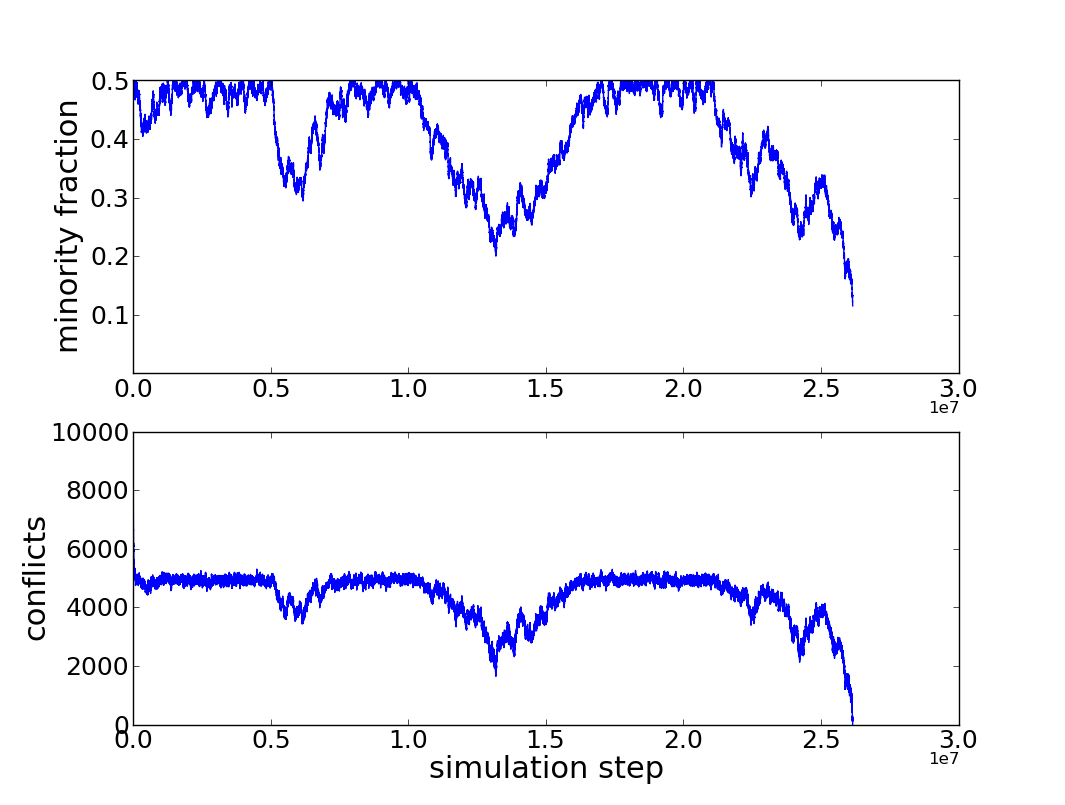
\includegraphics[height=65mm]{vmDynamics}
  \caption{Evolution of conflicts and minority fraction in a single voting model simulation.}
  \label{fig:vmDynamics}
\end{figure}

\begin{figure}
  \centering
  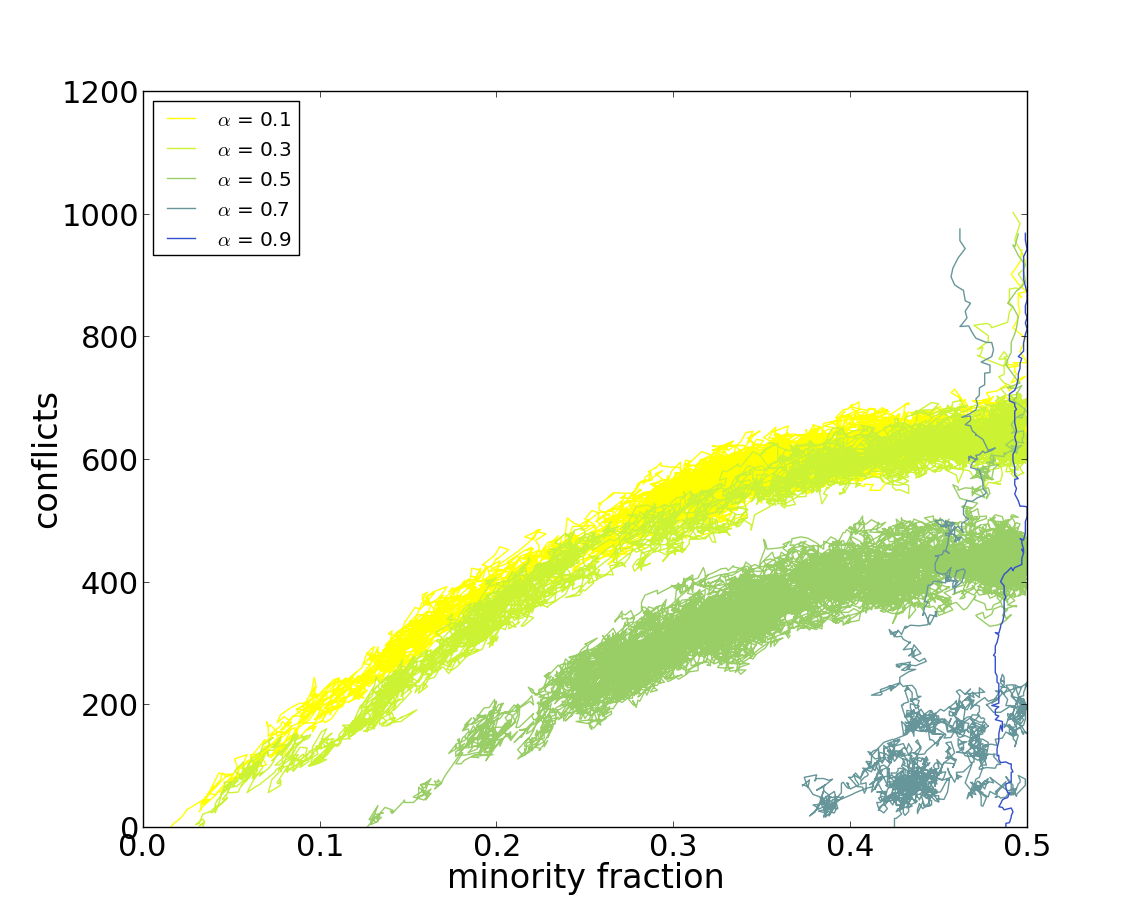
\includegraphics[height=65mm]{vmPhasePortrait}
  \caption{Phase portrait at varying values of $\alpha$.}
  \label{fig:vmPP}
\end{figure}

\begin{figure}
  \centering
  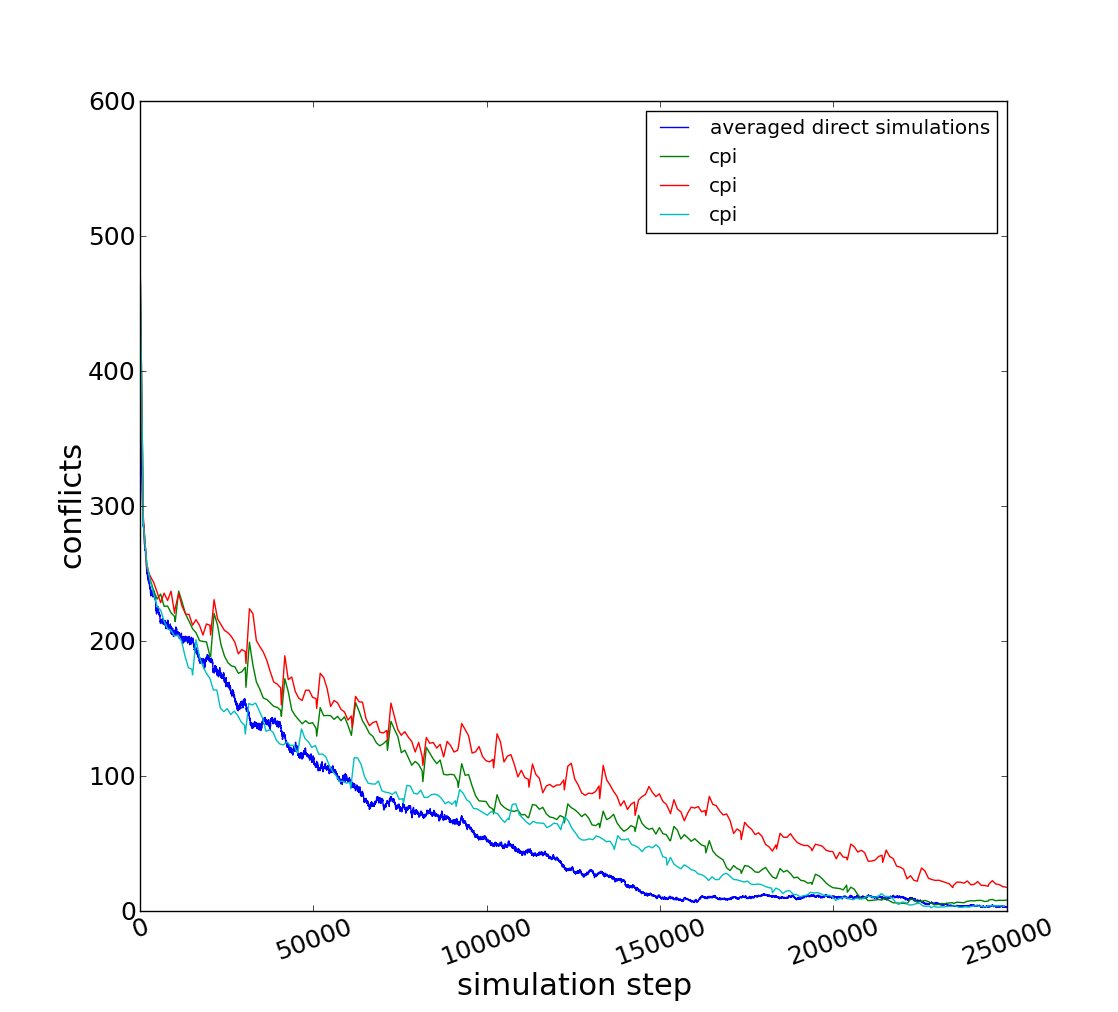
\includegraphics[height=65mm]{vmHealing}
  \caption{``Healing'' of voting model back to slow manifold, simulation was restricted and immediately lifted every $10,000$ steps.}
  \label{fig:vmHealing}
\end{figure}

\begin{figure}
  \centering
  \includegraphics[height=65mm]{vmCPISlow}
  \caption{First CPI method in which finished runs in the ensemble are entirely removed from the simulation. This causes slower convergence.}
  \label{fig:vmSlow}
\end{figure}

\begin{figure}
  \centering
  \includegraphics[height=65mm]{vmCPIFast}
  \caption{Second CPI method in which finished runs in the ensemble contribute their data to the projection step, but are no longer evolved in time. As this amounts to added zero conflict runs to the ensemble, convergence is faster}
  \label{fig:vmSlow}
\end{figure}

\begin{figure}
  \centering
  \subfloat[Only includes runs that have reached consensus]{
    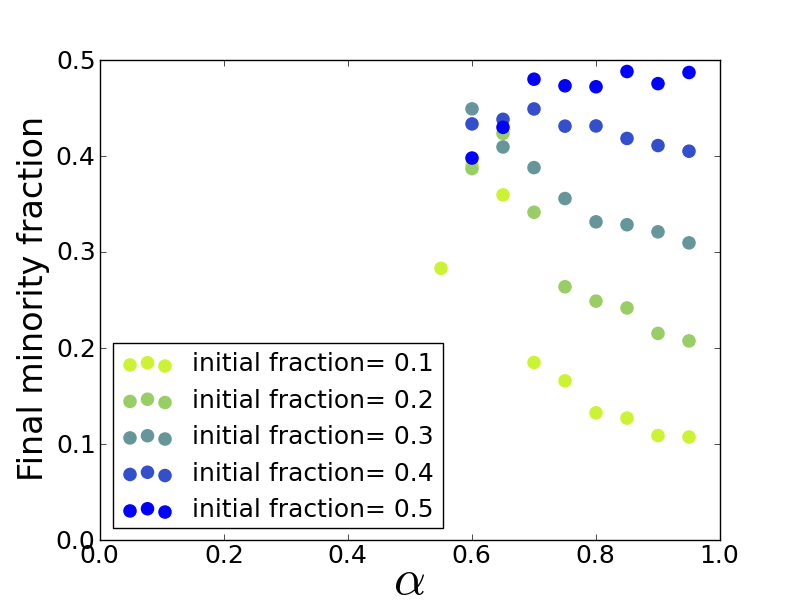
\includegraphics[width=72mm]{bifData_same_1000_4}
    \label{fig:rwSameA}
  }
  \hspace{3mm}
  \subfloat[Includes all runs, even if conflicts exist at the simulation's end] {
    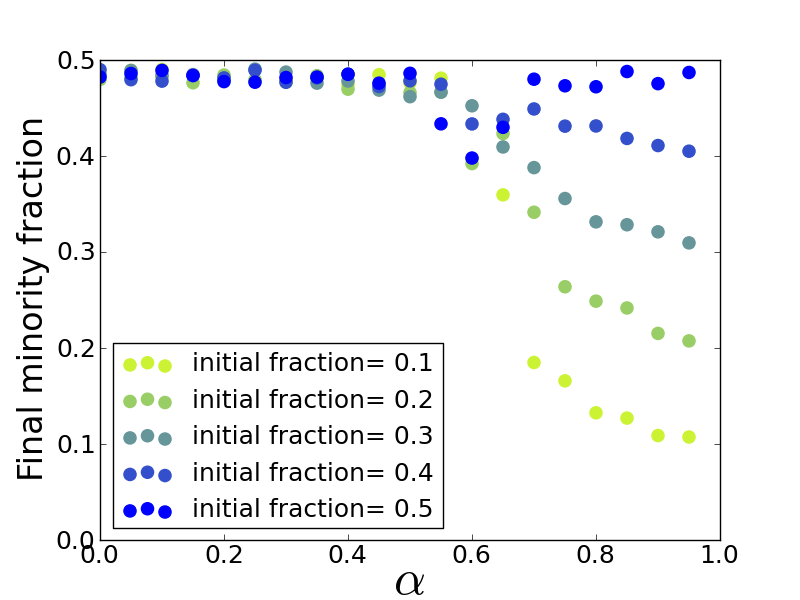
\includegraphics[width=72mm]{bifData_noConvergence_same_1000_4}
    \label{fig:rwSameB}
  }
  \caption{Final minority fraction as a function of $\alpha$ and initial minority fraction (rewire-to-same), results from our data.}
  \label{fig:myRWtoSameBD}
\end{figure}

\end{document}
